\documentclass{beamer}
\usepackage{beamerthemeshadow}
%\usepackage{beamercolorthemedolphin}
\usepackage{lastpage}

\usepackage{xcolor}
\usepackage{pgf}

\newcommand{\bi}{\begin{itemize}}
\newcommand{\ei}{\end{itemize}}
\newcommand{\be}{\begin{enumerate}}
\newcommand{\ee}{\end{enumerate}}
\newcommand{\bd}{\begin{description}}
\newcommand{\ed}{\end{description}}
\newcommand{\prbf}[1]{\textbf{#1}}
\newcommand{\prit}[1]{\textit{#1}}
\newcommand{\beq}{\begin{equation}}
\newcommand{\eeq}{\end{equation}}
\newcommand{\bdm}{\begin{displaymath}}
\newcommand{\edm}{\end{displaymath}}

\newcommand{\ft}[1]{
  \frametitle{\begin{tabular}{p{4in}r} \textcolor{white}{#1} & \small{\textcolor{white}{\thepage$~$ / \pageref{LastPage}}}\end{tabular}}
  \setbeamercovered{transparent=18}
}

\newcommand{\stepinv}{\setbeamercovered{invisible}}
\newcommand{\stopinv}{\setbeamercovered{transparent=18}}
\newcommand{\uncoverinv}[1]
{
  \setbeamercovered{invisible}
  \uncover<+->{#1}
  \setbeamercovered{transparent=18}
}
\newcommand{\ans}[1]{\textcolor{blue}{#1}}
\newcommand{\ansinv}[1]
{
  \setbeamercovered{invisible}
  \uncover<+->{\textcolor{blue}{#1}}
  \setbeamercovered{transparent=18}
}
\newcommand{\setinv}{\setbeamercovered{invisible}}
\newcommand{\setvis}{\setbeamercovered{transparent=18}}
\newcommand{\centerpic}[2]
{
  \begin{center}
  \includegraphics[#1]{#2}
  \end{center}
}
\newcommand{\h}[1]{\hat{#1}}
\newcommand{\ds}{\displaystyle}

\definecolor{mycolor}{rgb}{0.125,0.5,0.05}
\usecolortheme[named=mycolor]{structure}

\title[Empirical Significance of Learning with Firm-Specific Capital]{Empirical Significance of Learning in a New Keynesian Model with Firm-Specific Capital}
\author[Jordan River Conference. Indiana University. April 2007.]{James Murray}
\date{April 20, 2007}

\begin{document}

\frame{\titlepage}
\setcounter{page}{1}

\frame{
  \ft{Introduction}
  \bi
  \item Purpose: 
    \bi
    \item Estimate the empirical significance of learning.
    \item Determine what features of U.S. data (if any) learning can explain.
    \ei
  \item Learning may deliver features:
    \bi
    \item Orphanides and Williams (2005): ``Inflation scares''.
    \item Milani (2005): Persistence.
    \item Volatility persistence.
    \item Bullard and Singh (2007), Primiceri (2005): Great Moderation.
    \ei
  \item Estimate a NK model with learning and RE by MLE.
  \item Examine forecast errors, evolution of shocks, and evolution of expectations.
  \ei
}

\frame
{
  \ft{Consumers}
  \textbf{Utility function:}
  \bdm U_0 = E_0^* \sum_{t=0}^{\infty} \beta^t \left[ \frac{1}{1-\sigma} \xi_t \left(c_t(i) - \eta c_{t-1}(i)\right)^{1-\sigma} - \frac{1}{1+\mu} n_t(i)^{1+\mu} \right] \edm
  \bi
  \item $E_t^*$: possibly non-rational expectations operator.
  \item $c_t(i)$: consumption at time $t$. 
  \item $n_t(i)$: labor supply at time $t$.
  \item $\xi_t$: common preference shock.
  \item $\beta$: discount factor.
  \item $\sigma \in (0,\infty)$: related to the intertemporal elasticity of substitution.
  \item $\eta \in [0,1)$: degree of habit formation.
  \ei
}

\frame
{
  \ft{Production}
  \textbf{Final good production:}
  \bdm y_t = \left[ \int_0^1 y_t(i)^{\frac{\theta-1}{\theta}} di \right]^{\frac{\theta}{\theta-1}} \edm
  \bi
  \item $y_t$ output of final good, $y_t(i)$ output of intermediate good $i$.
  \item $\theta \in (1,\infty)$: elasticity of substitution in production.
  \ei
  \textbf{Intermediate goods production:}
  \bdm y_t(i) = z_t k_t(i)^{\alpha} n_t(i)^{1-\alpha} \edm
  \bi
  \item $z_t$: common technology shock.
  \item $k_t(i)$: firm-specific capital good.
  \ei
}

\frame
{
  \ft{Sticky prices}
  \bi
  \item Follow Calvo (1983) pricing: fraction $1-\omega$ firms re-optimize their price each period.
  \item Inflation indexation: Those who cannot re-optimize may adjust according to:
    \bdm p_{t}(i) = p_{t-1}(i) + \gamma \pi_{t-1} \edm
  \item Even with endogenous capital (Woodford, 2005), leads to Phillips curve:
  \bdm \pi_t = \frac{\gamma}{1+\beta\gamma} \pi_{t-1} +  \frac{\beta}{1+\beta\gamma} E_t^* \pi_{t+1} + \kappa \h{s}_t \edm
  \item $\h{s}_t$: average marginal cost in the economy (percentage deviation from steady state).
  \item $\kappa$: function of many parameters.
  \ei
}

\frame
{
  \ft{Firm-Specific Investment}
  \bi
  \item Final good is converted to a firm-specific capital good.
  \item Investment of $I_t(i)$ leads to capital stock next period:
  \ei
  \bdm k_{t+1}(i) = (1-\delta) k_t(i) + \mu_t I_t(i) - \frac{\phi}{2} \left[\frac{k_{t+1}(i)}{k_t(i)} - 1 \right]^2 k_t(i) \edm
  \bi
  \item $\mu_t$: common investment technology shock.
  \item $\delta$: depreciation rate.
  \item $\phi$: capital adjustment cost parameter.
  \ei
}

\frame
{
  \ft{Rest of the model}
  \bi
  \item Market clearing condition: $\ds y_t = c_t + I_t$
  \item Monetary policy: $\h{r}_t = \rho_r \h{r}_{t-1} + (1-\rho_r) \left(\psi_{\pi} \pi_t + \psi_y \h{y}_t \right) + \epsilon_{r,t}$
    \bi
    \item $\psi_{\pi} \in (0,\infty)$: feedback on inflation.
    \item $\psi_{y} \in (0,\infty)$: feedback on output.
    \item $\rho_r \in (0,1)$: smoothing parameter.
    \ei
  \item Non-policy shocks (percentage deviations from steady state) are AR(1):
    \bi
    \item Preference shock: $\h{\xi}_t = \rho_{\xi} \h{\xi}_{t-1} + \epsilon_{\xi,t}$ 
    \item Technology shock: $\h{z}_t = \rho_{z} \h{z}_{t-1} + \epsilon_{z,t}$ 
    \item Investment shock: $\h{\mu}_t = \rho_{\mu} \h{\mu}_{t-1} + \epsilon_{\mu,t}$ 
    \ei
  \ei
}

\frame
{
  \ft{Learning in DSGEs}
  Suppose a DSGE model of the form:
  \bdm \Omega_{0} x_t = \Omega_{1} x_{t-1} + \Omega_{2} E_t^* x_{t+1} + \Psi \epsilon_t \edm
  \bi
  \item $x_t$ vector of time $t$ variables, all observable to agents.
  \item $E_t^*$: possibly non-rational expectations operator.
  \ei
  \vspace{1pc}
  Rational expectations solution implies:
  \bdm E_t x_{t+1} = G x_t \edm
  \bi
  \item Agents know the form of this solution, but estimate elements of $G$ by least squares.
  \item Use as explanatory variables past observations of $x_t^k$.
  \item $x_t^k$ includes a constant and all variables in $x_t$ where the associated column in $G$ is non-zero.
  \ei
}
  
\frame
{
  \ft{Ordinary Least Squares}
  \bi 
  \item Let $G_t^k$ include non-zero columns of $G$ and a constant.
  \item Ordinary least squares estimate for $G^k$ at time $t$:
    \bdm \left(\hat{G}_t^k\right)' = \left( \frac{1}{t-1} \sum_{\tau=1}^{t-1} x_{\tau-1}^k {x_{\tau-1}^{k}}' \right)^{-1} \left( \frac{1}{t-1} \sum_{\tau=1}^{t-1} x_{\tau-1}^k x_{\tau}' \right) \edm
  \item Least squares forecast:
    \beq \label{eq:agfore} E_t^* x_{t+1} = \h{g}_{0,t} + \h{G}_t E_t^* x_t = (I + \h{G}_t)\h{g}_{0,t} + \h{G}_t^2 x_{t-1} \eeq
  \item Evolution of $\h{G}_t^k$ in recursive form:
    \beq \label{eq:lnG} \hat{G}_t^k = \hat{G}_{t-1}^k + g (x_{t-1} - \hat{G}_{t-1}^k x_{t-2}^k) {x_{t-2}^k}' R_t^{-1} \eeq
    \beq \label{eq:lnX} R_t = R_{t-1} + g (x_{t-2}^k {x_{t-2}^k}' - R_{t-1}) \eeq
  \item where $g=1/(t-1)$ is the learning gain.
  \ei
}

\frame
{
  \ft{Constant Gain Learning}
  \bi
  \item Ordinary least squares $\rightarrow$ learning dynamics disappear as $t$ grows.
  \item Constant gain: assumes $g$ is constant.
  \item With a constant gain, learning dynamics persist in the long run.
  \item Dynamics of expectations depend on the size of the constant learning gain.
  \item Appropriate initial condition + $(g=0)$ $\rightarrow$ RE.
  \item Standard statistical test for $g=0$ can conclude a rejection failure to RE.
  \ei
}

\frame
{
  \ft{Estimation Procedure}
  Estimate by MLE using Kalman filter (Hamilton, 1994).
  \bi
  \item State equation: 
    \beq \label{eq:alm} x_t = \Omega_0^{-1}\Omega_{2}\left(I+\h{G}_t\right)\h{g}_{0,t} + \Omega_0^{-1} \left(\Omega_{1} + \Omega_{2} \h{G}_t^2 \right) x_{t-1}  + \Omega_0^{-1} \Psi \epsilon_t. \eeq
  \item Observation equations:
    \bdm \begin{array}{c} 
      \ds GDP_t^g = 100\left(\h{y}_t - \h{y}_{t-1}\right) \\
      \ds I_t^g = 100\left(\h{I}_t - \h{I}_{t-1}\right) \\
      \ds INF_t = \pi^{*} + 400\pi_t \\
      \ds FF_t = r^{*} + 400\h{r}_t
    \end{array}
    \edm
  \item Initialize Kalman filter and learning algorithm with the MSV solution under RE.
  \ei
}

\frame
{
\ft{Results with No Capital Accumulation}
\begin{table}[ht]
\begin{scriptsize}
\begin{center}
\begin{tabular}{|l|c|r@{.}l|r@{.}l|} \hline
Description & Parameter & \multicolumn{2}{|c|}{Learning} & \multicolumn{2}{|c|}{RE} \\ \hline
Learning gain & $g$ & 0&017225*** & \multicolumn{2}{|c|}{--} \\ 
Discount factor & $\beta$ & 0&994528*** & 0&994893*** \\ 
Habit formation & $\eta$ & 0&269967** & 0&213315 \\ 
Inverse elasticity sub. & $\sigma$ & 16&264823 & 17&589033 \\ 
Elasticity of sub. production & $\theta$ & 11&459122 & 10&030577 \\ 
Inverse elasticity labor supply & $\mu$ & 2&509288 &  1&791766 \\ 
Calvo parameter & $\omega$ & 0&715756 & 0&713950 \\ 
Inflation indexation & $\gamma$ & 0&441247*** & 0&958006*** \\ 
MP interest rate smoothing & $\rho_r$ & 0&866560*** & 0&823025*** \\ 
MP feedback on output & $\psi_y$ & 0&123166** & 0&055319* \\ 
MP feedback on inflation & $\psi_{\pi}$ & 0&995049*** & 1&067211*** \\ 
Pref. shock persistence & $\rho_{\xi}$ & 0&931082*** & 0&962095***  \\ 
Tech. shock persistence & $\rho_{z}$ & 0&000010 & 0&000010 \\ 
Steady state inflation & $\pi^{*}$ & 2&814514*** & 3&296221** \\ 
Std. dev. technology shock & $\sigma_z$ & 0&301741* & 0&340167 \\ 
Std. dev. preference shock & $\sigma_{\xi}$ & 0&280402* & 0&254504 \\ 
Std. dev. interest rate shock & $\sigma_{r}$ & 0&002283*** & 0&002344*** \\ \hline
\end{tabular}

* Significantly different from zero at the 10\% level.\newline
** Significantly different from zero at the 5\% level.\newline
*** Significantly different from zero at the 1\% level.\newline
\end{center}
\end{scriptsize}
\end{table}
}


\frame
{
  \ft{Results with No Capital Accumulation}
  \bi
  \item Learning statistically significant.
  \item Learning leads to lower degree of inflation indexation.
  \item Habit formation still significant source of persistence.
  \item Very similar estimates for the degree of price flexibility.
  \item Possible reasons for differences with Milani (2005):
    \bi
    \item MLE vs. Bayesian methods.
    \item Different initial condition for recursive learning process.
    \item Different data: Growth rate of real GDP vs. CBO measure of output gap.
    \ei
  \ei
}

\frame
{
  \ft{In-Sample One Quarter Ahead Forecast Errors}
  \begin{center}
  \vspace*{-0.1in}\hspace*{-0.24in}\begin{tabular}{ccc}
  \multicolumn{3}{c}{\textbf{Learning}}  \\
  \small{Output} & \small{Inflation} & \small{Interest Rate} \\
  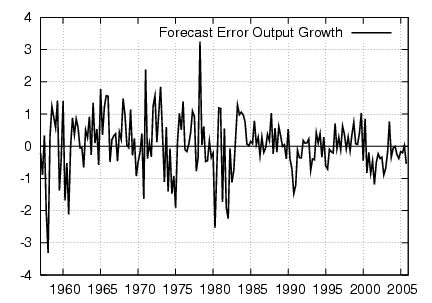
\includegraphics[scale=0.23]{plots/ln_nocap_full_res_yfe.png} & 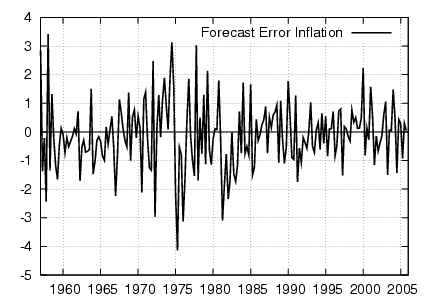
\includegraphics[scale=0.23]{plots/ln_nocap_full_res_pife.png} & 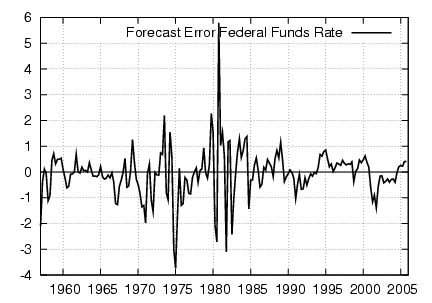
\includegraphics[scale=0.23]{plots/ln_nocap_full_res_rfe.png} \\ \\
  \multicolumn{3}{c}{\textbf{Rational Expectations}}  \\
  \small{Output} & \small{Inflation} & \small{Interest Rate} \\
  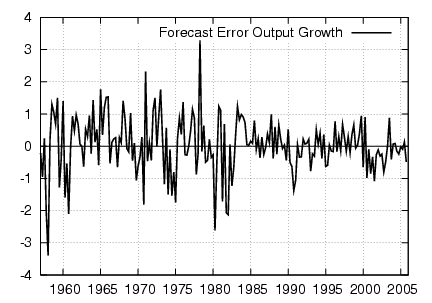
\includegraphics[scale=0.23]{plots/re_nocap_full_res_yfe.png} & 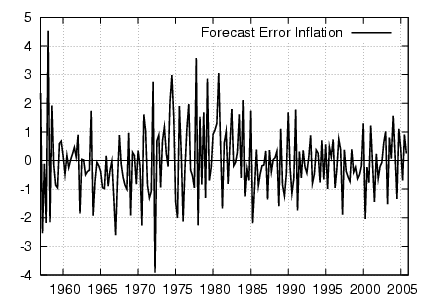
\includegraphics[scale=0.23]{plots/re_nocap_full_res_pife.png} & 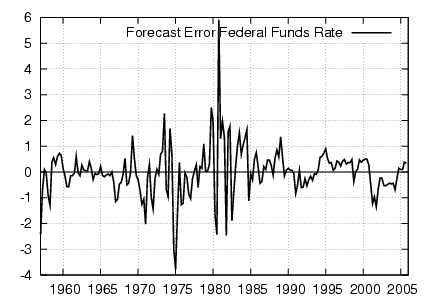
\includegraphics[scale=0.23]{plots/re_nocap_full_res_rfe.png} \\ \\ \\
  \end{tabular}
  \end{center}
}

\frame
{
  \ft{In-Sample One Quarter Ahead Forecast Errors}
  \bi
  \item Forecast errors are very similar for Learning and RE.
  \item Forecast errors are more volatile in 1970s.
  \item Huge forecast errors for federal funds rate in late 70s, early 80s.
  \item Learning appears not to be explaining U.S. dynamics better than RE.
  \item Both fail to explain high volatility in 70s with low volatility after mid 80s.
  \ei
}

\frame
{
  \ft{Eight Quarter Out-of-Sample Forecasts}
  \bi
  \item Estimate the model through 1989:Q4.
  \item Use estimated parameters to forecast 1990:Q1 - 2005:Q4.
  \item For each quarter, forecast eight periods ahead.
  \item Given forecasts of each horizon, compute MSE.
  \item Do the same for a VAR(4) and Litterman (1986) BVAR(4).
  \ei
}

\frame
{
  \ft{Eight Quarter Out-of-Sample Forecasts}
  \begin{center}
  \begin{tabular}{ccc}
  Output & Inflation  \\ 
  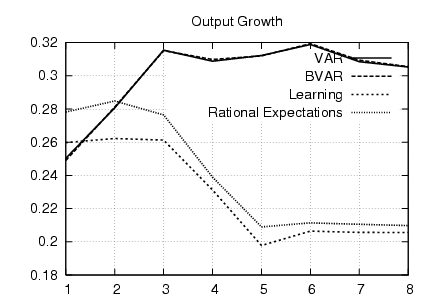
\includegraphics[scale=0.3]{plots/mse_nocap_y.png} & 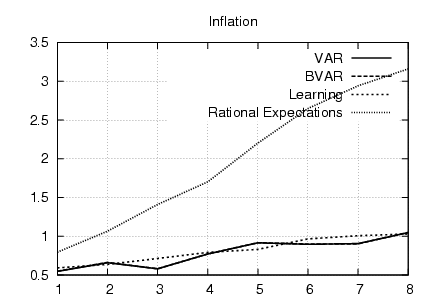
\includegraphics[scale=0.3]{plots/mse_nocap_pi.png} \\
  Interest Rate & \\
  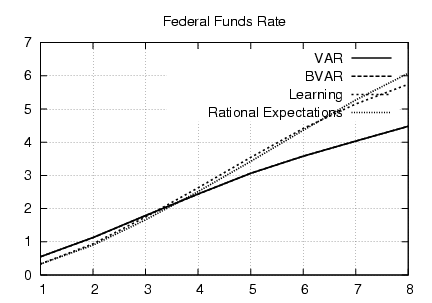
\includegraphics[scale=0.3]{plots/mse_nocap_r.png} & \\
  \end{tabular}
  \end{center}
}

\frame
{
  \ft{Smoothed Technology Shocks}
  \begin{center}
  \vspace*{-0.1in}\hspace*{-0.24in}\begin{tabular}{ccc}
  \multicolumn{3}{c}{\textbf{Learning}}  \\
  \small{Technology Shock} & \small{Preference Shock} & \small{Interest Rate Shock} \\
  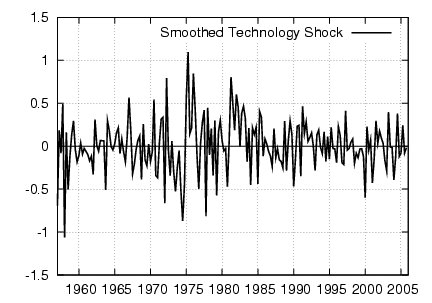
\includegraphics[scale=0.23]{plots/ln_nocap_full_res_techsh.png} & 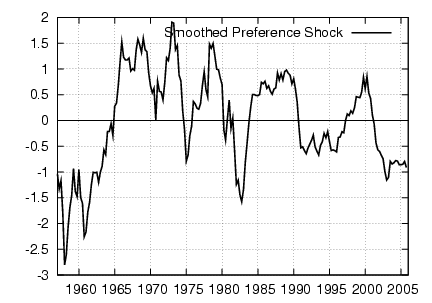
\includegraphics[scale=0.23]{plots/ln_nocap_full_res_prefsh.png} & 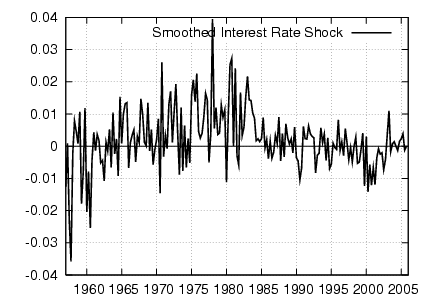
\includegraphics[scale=0.23]{plots/ln_nocap_full_res_ffsh.png} \\ \\
  \multicolumn{3}{c}{\textbf{Rational Expectations}}  \\
  \small{Technology Shock} & \small{Preference Shock} & \small{Interest Rate Shock} \\
  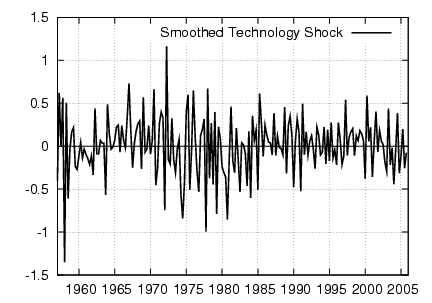
\includegraphics[scale=0.23]{plots/re_nocap_full_res_techsh.png} & 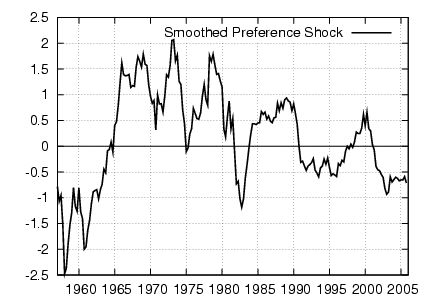
\includegraphics[scale=0.23]{plots/re_nocap_full_res_prefsh.png} & 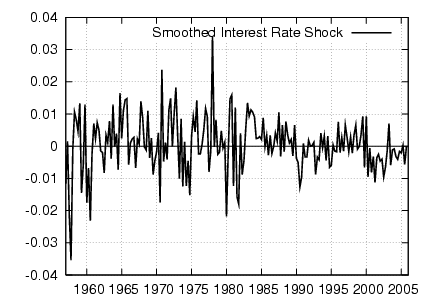
\includegraphics[scale=0.23]{plots/re_nocap_full_res_ffsh.png} \\ \\ \\
  \end{tabular}
  \end{center}
}

\frame
{
  \ft{Agents' Expectations}
  \begin{center}
  \vspace*{-0.1in}\hspace*{-0.24in}\begin{tabular}{ccc}
  \multicolumn{3}{c}{\textbf{Learning}}  \\
  \small{Consumption} & \small{Inflation} & \small{Preference shock} \\
  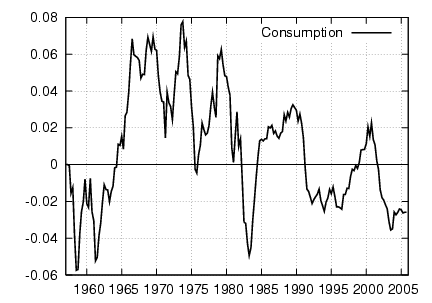
\includegraphics[scale=0.23]{plots/ln_nocap_full_res_cag.png} & 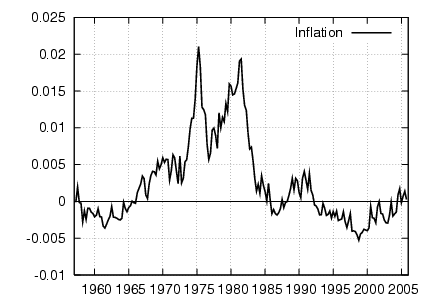
\includegraphics[scale=0.23]{plots/ln_nocap_full_res_piag.png} & 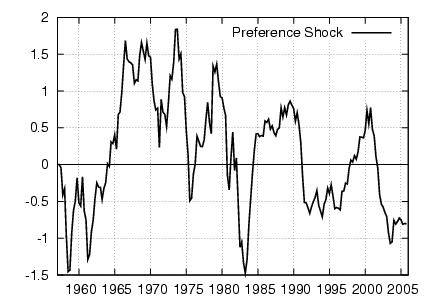
\includegraphics[scale=0.23]{plots/ln_nocap_full_res_xiag.png} \\ \\
  \multicolumn{3}{c}{\textbf{Rational Expectations}}  \\
  \small{Consumption} & \small{Inflation} & \small{Preference shock} \\
  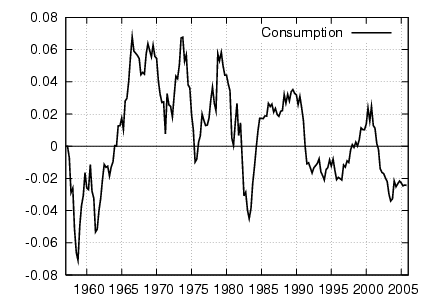
\includegraphics[scale=0.23]{plots/re_nocap_full_res_cag.png} & 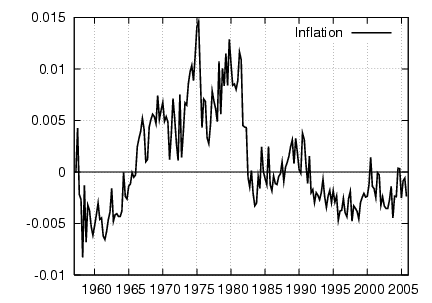
\includegraphics[scale=0.23]{plots/re_nocap_full_res_piag.png} & 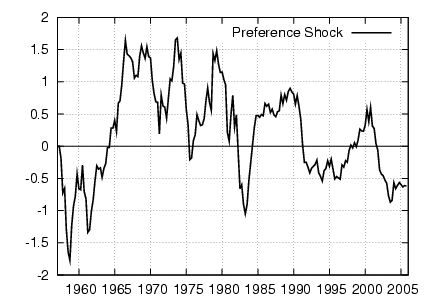
\includegraphics[scale=0.23]{plots/re_nocap_full_res_xiag.png} \\ \\ \\
  \end{tabular}
  \end{center}
}

\frame
{
\ft{Results with Endogenous Capital Accumulation}
\begin{table}[ht]
\begin{scriptsize}
\begin{center}
\begin{tabular}{|l|c|r@{.}l|r@{.}l|} \hline
Description & Parameter & \multicolumn{2}{|c|}{Learning} & \multicolumn{2}{|c|}{RE} \\ \hline
Learning gain & $g$ & 0&024327** & \multicolumn{2}{|c|}{--} \\ 
Discount factor & $\beta$ & 0&993366*** & 0&992763*** \\ 
Habit formation & $\eta$ & 0&281563** & 0&286030* \\ 
Inverse elasticity sub. & $\sigma$ & 18&558950 & 16&328695 \\ 
Elasticity of sub. production & $\theta$ & 13&122359 & 7&317025 \\ 
Inverse elasticity labor supply & $\mu$ & 3&329474 & 6&219549 \\ 
Capital share of income & $\alpha$ & 0&174750 & 0&186636 \\ 
Depreciation rate & $\delta$ & 0&163489 & 0&299872 \\ 
Cost of adjusting capital & $\phi$ & 13&455016 & 11&558055 \\ 
Calvo parameter & $\omega$ & 0&658099 & 0&774919 \\ 
Inflation indexation & $\gamma$ & 0&404221*** & 0&760702*** \\ 
MP interest rate smoothing & $\rho_r$ & 0&869496*** & 0&859279*** \\ 
MP feedback on output & $\psi_y$ & 0&064696* & 0&128857*** \\ 
MP feedback on inflation & $\psi_{\pi}$ & 0&992672*** & 0&967512*** \\ 
Pref. shock persistence & $\rho_{\xi}$ & 0&984689*** & 0&980813***  \\ 
Tech. shock persistence & $\rho_{z}$ & 0&012960 & 0&000010 \\ 
Inv. shock persistence & $\rho_{\mu}$ & 0&804935*** & 0&824007*** \\ 
Steady state inflation & $\pi^{*}$ & 3&570552*** & 4&073905*** \\ 
Std. dev. technology shock & $\sigma_z$ & 0&229175** & 0&400000** \\ 
Std. dev. investment shock & $\sigma_{\mu}$ & 0&060246*** & 0&052502***  \\ 
Std. dev. preference shock & $\sigma_{\xi}$ & 0&231848* & 0&214337* \\ 
Std. dev. interest rate shock & $\sigma_{r}$ & 0&002291*** & 0&002286*** \\ \hline
\end{tabular}
\end{center}
\end{scriptsize}
\end{table}
}

\frame
{
  \ft{Results with Endogenous Capital Accumulation}
  \bi
  \item Learning remains statistically significant.
  \item Including capital leads to a lower degree of inflation indexation.
  \item Learning further lowers the degree of inflation indexation.
  \item Habit formation still significant source of persistence.
  \item Learning leads to lower estimates for the degree of price flexibility.
  \item Learning leads to lower estimates for the variance of the technology shock.
  \ei
}

\frame
{
  \ft{One Quarter Ahead Forecast Errors}
  \begin{center}
  \hspace*{-0.32in}\begin{tabular}{cccc}
  \multicolumn{4}{c}{\textbf{Learning}}  \\
  \small{Output} & \small{Investment} & \small{Inflation} & \small{Interest Rate} \\
  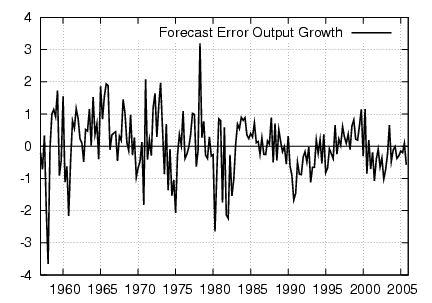
\includegraphics[scale=0.18]{plots/ln_cap_full_res_yfe.png} & 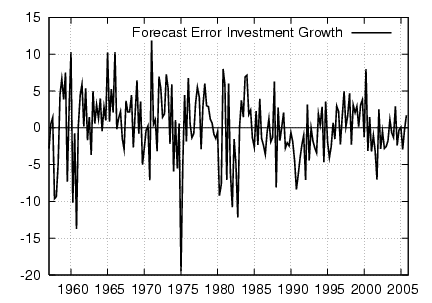
\includegraphics[scale=0.18]{plots/ln_cap_full_res_Ife.png} & 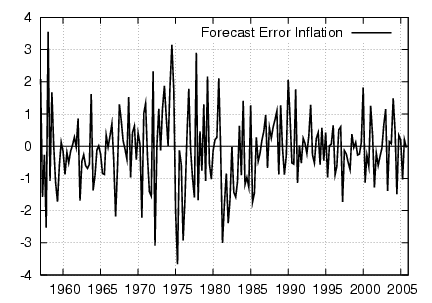
\includegraphics[scale=0.18]{plots/ln_cap_full_res_pife.png} & 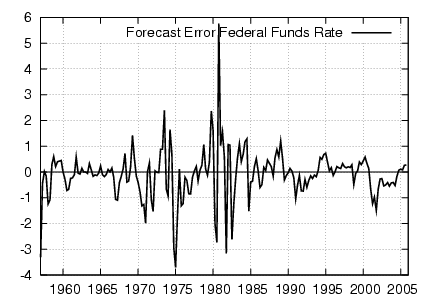
\includegraphics[scale=0.18]{plots/ln_cap_full_res_rfe.png} \\ \\
  \multicolumn{4}{c}{\textbf{Rational Expectations}}  \\
  \small{Output} & \small{Investment} & \small{Inflation} & \small{Interest Rate} \\
  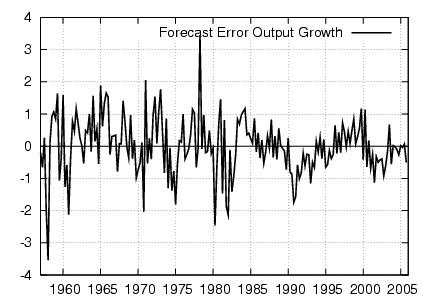
\includegraphics[scale=0.18]{plots/re_cap_full_res_yfe.png} & 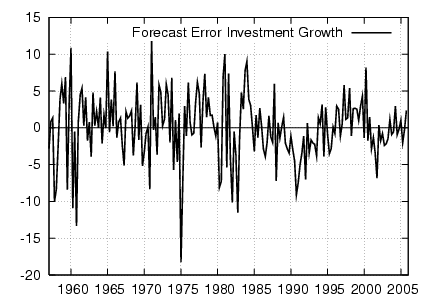
\includegraphics[scale=0.18]{plots/re_cap_full_res_Ife.png} & 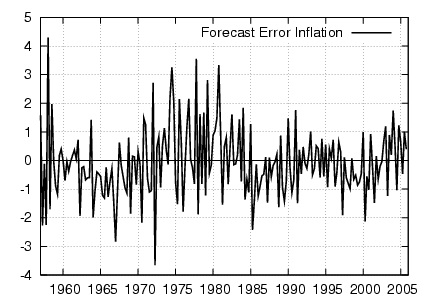
\includegraphics[scale=0.18]{plots/re_cap_full_res_pife.png} & 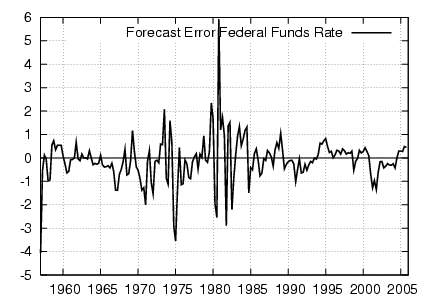
\includegraphics[scale=0.18]{plots/re_cap_full_res_rfe.png} \\ \\ \\
  \end{tabular}
  \end{center}
}

\frame
{
  \ft{Eight Quarter Out-of-Sample Forecasts}
  \begin{center}
  \begin{tabular}{ccc}
  Output & Inflation  \\ 
  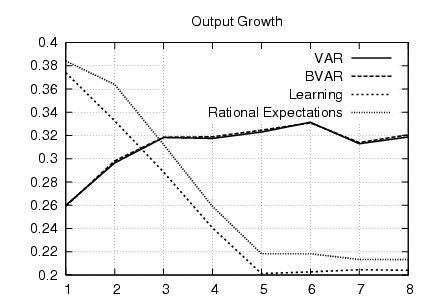
\includegraphics[scale=0.3]{plots/mse_cap_y.png} & 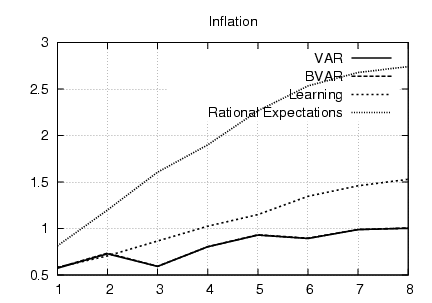
\includegraphics[scale=0.3]{plots/mse_cap_pi.png} \\
  Investment & Interest Rate \\
  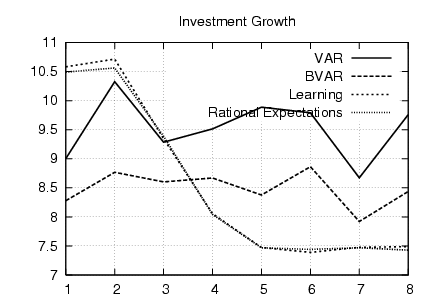
\includegraphics[scale=0.3]{plots/mse_cap_I.png} & 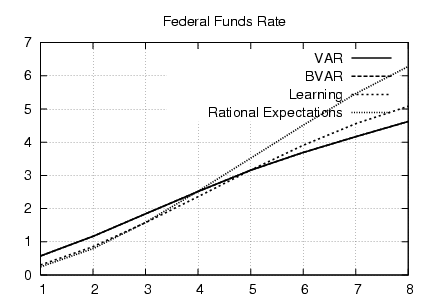
\includegraphics[scale=0.3]{plots/mse_cap_r.png} \\
  \end{tabular}
  \end{center}
}

\frame
{
  \ft{Smoothed Technology Shocks}
  \begin{center}
  \hspace*{-0.32in}\begin{tabular}{cccc}
  \multicolumn{4}{c}{\textbf{Learning}}  \\
  \small{Technology Shock} & \small{Investment Shock} & \small{Preference Shock} & \small{Interest Rate Shock} \\
  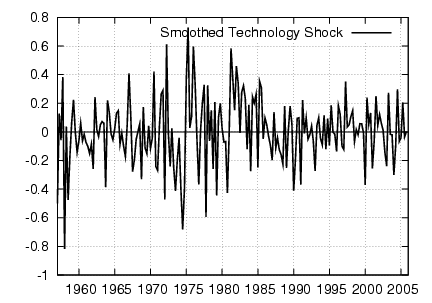
\includegraphics[scale=0.18]{plots/ln_cap_full_res_techsh.png} & 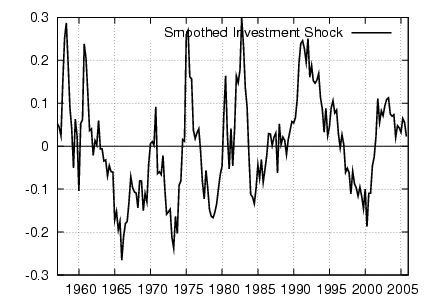
\includegraphics[scale=0.18]{plots/ln_cap_full_res_invsh.png} & 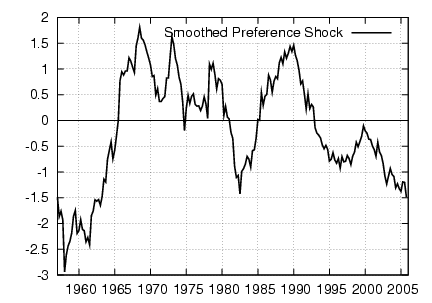
\includegraphics[scale=0.18]{plots/ln_cap_full_res_prefsh.png} & 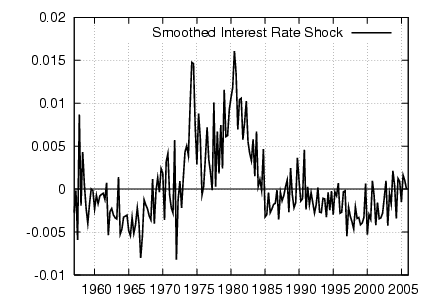
\includegraphics[scale=0.18]{plots/ln_cap_full_res_ffsh.png} \\ \\
  \multicolumn{4}{c}{\textbf{Rational Expectations}}  \\
  \small{Technology Shock} & \small{Investment Shock} & \small{Preference Shock} & \small{Interest Rate Shock} \\
  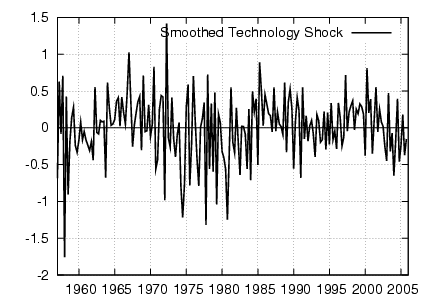
\includegraphics[scale=0.18]{plots/re_cap_full_res_techsh.png} & 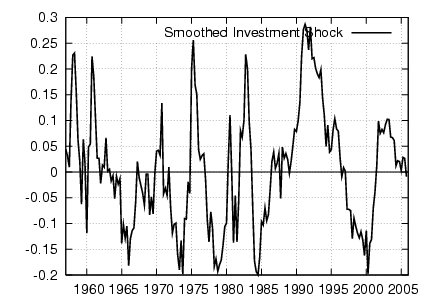
\includegraphics[scale=0.18]{plots/re_cap_full_res_invsh.png} & 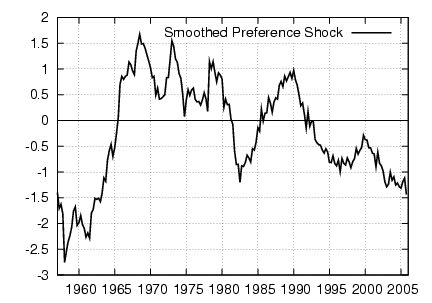
\includegraphics[scale=0.18]{plots/re_cap_full_res_prefsh.png} & 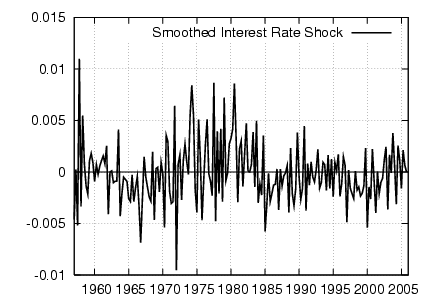
\includegraphics[scale=0.18]{plots/re_cap_full_res_ffsh.png} \\ \\ \\
  \end{tabular}
  \end{center}
}


\frame
{
  \ft{Agents' Expectations}
  \begin{center}
  \vspace*{-0.1in}\hspace*{-0.24in}\begin{tabular}{ccc}
  \multicolumn{3}{c}{\textbf{Learning}}  \\
  \small{Consumption} & \small{Inflation} & \small{Capital stock} \\
  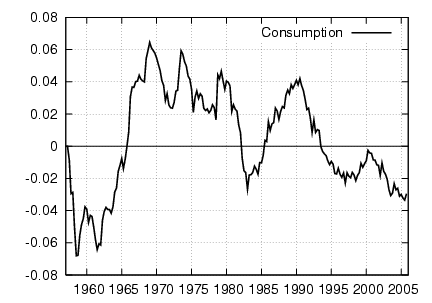
\includegraphics[scale=0.23]{plots/ln_cap_full_res_cag.png} & 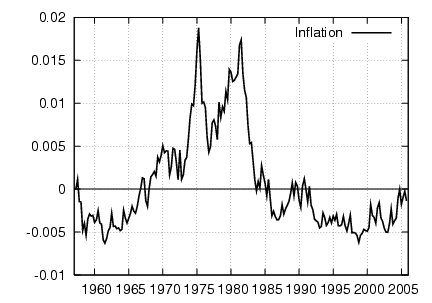
\includegraphics[scale=0.23]{plots/ln_cap_full_res_piag.png} & 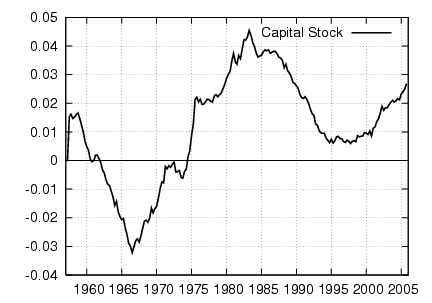
\includegraphics[scale=0.23]{plots/ln_cap_full_res_kag.png} \\ \\
  \multicolumn{3}{c}{\textbf{Rational Expectations}}  \\
  \small{Consumption} & \small{Inflation} & \small{Capital stock} \\
  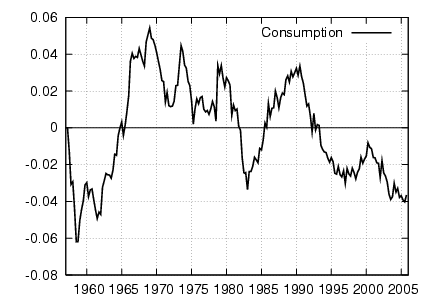
\includegraphics[scale=0.23]{plots/re_cap_full_res_cag.png} & 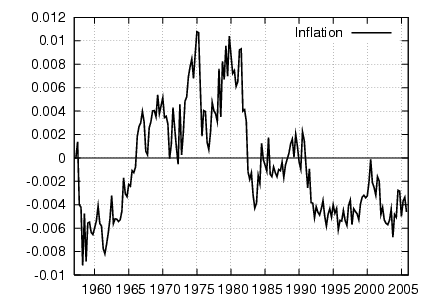
\includegraphics[scale=0.23]{plots/re_cap_full_res_piag.png} & 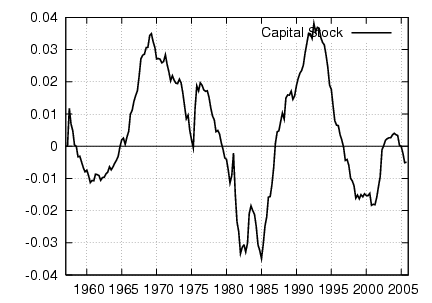
\includegraphics[scale=0.23]{plots/re_cap_full_res_kag.png} \\ \\ \\
  \end{tabular}
  \end{center}
}

\frame
{
  \ft{Conclusion}
  \bi
  \item Learning successes:
    \bi
    \item Lower estimates for inflation indexation.
    \item Lower estimates for the Calvo parameter (using capital).
    \item Lower estimates for variance of the technology shock (using capital).
    \item Some evidence of inflation scares.
    \item Better performance out-of-sample, especially for inflation.
    \ei
  \item Learning failures:
    \bi
    \item Very similar to RE in explaining the data.
    \item 1970s inflation, monetary policy.
    \ei
  \ei
}


\end{document}

